% !TEX encoding = UTF-8
% !TEX TS-program = pdflatex
% !TEX root = ../tesi.tex

%**************************************************************
\chapter{Lo stage}
\label{cap:descrizione-stage}
%**************************************************************

\section{Pianificazione}
Prima dell'inizio del progetto, ho redatto assieme al tutor aziendale un piano di lavoro, all'interno del quale ho riportato gli obiettivi individuati, la pianificazione del lavoro sotto forma di processi, suddivisi a loro volta in attività, ad ognuna delle quali sono state assegnate delle ore di lavoro, la cui somma sarà il totale delle ore a disposizione per lo stage.

\bigskip

%% !TEX encoding = UTF-8
% !TEX TS-program = pdflatex
% !TEX root = ../tesi.tex

% Tabella da personalizzare in base alle ore delle attività

\begin{tabularx}{\textwidth}{|c|X|}
	\hline
	\textbf{Durata in ore} & \textbf{Descrizione dell'attività} \\\hline
	
	\textbf{48} & \textbf{Formazione sulle tecnologie utilizzate} \\	 
    \hline
    
    \textbf{72} & \textbf{Definizione del sistema hardware/software e relativa documentazione} \\ \hdashline 
    \multirow{3}{0cm}\\ 
    \textit{16} & 
    \textit{Analisi del problema e del dominio applicativo} \\
    \textit{26} & 
    \textit{Adattamento e revisione della piattaforma esistente} \\
    \textit{8} & 
    \textit{Test piattaforma hardware} \\
    \textit{18} & 
    \textit{Progettazione e sviluppo software CRM} \\
    \textit{4} & 
    \textit{Stesura documentazione} \\
    \hline
    
    \textbf{24} & \textbf{Modellazione e Stampa 3D}  \\ \hdashline 
    \multirow{4}{0cm}\\ 
    \textit{18} & 
    \textit{Design e modellazione involucro} \\
    \textit{6} & 
    \textit{Slicing del modello e stampa 3D} \\
    \hline
    
    \textbf{48} & \textbf{Sviluppo piattaforma online}  \\ \hdashline 
    \multirow{4}{0cm}\\ 
    \textit{18} & 
    \textit{Pianificazione e analisi dei requisiti} \\
    \textit{30} & 
    \textit{Sviluppo della piattaforma con iniziale attenzione al lato server} \\
    \hline
    
    \textbf{40} & \textbf{Cura dell'interfaccia grafica}  \\ 
    \hline
    
    \textbf{16} & \textbf{Test e verifica presenza bug}  \\
    \hline
    
	\textbf{48} & \textbf{Redazione dei manuali d'uso}  \\
    \hline    
    
    \textbf{12} & \textbf{Collaudo Finale}  \\ \hdashline 
    \multirow{4}{0cm}\\ 
    \textit{8} & 
    \textit{Collaudo} \\
    \textit{2} & 
    \textit{Incontro di presentazione della piattaforma con gli stakeholders} \\
    \textit{2} & 
    \textit{Live demo di tutto il lavoro di stage} \\
    \hline
	
	\textbf{Totale ore} & \multicolumn{1}{|c|}{\textbf{\totaleOre}} \\\hline
	
	
\end{tabularx} % tolta tabella in quanto sotto ho omesso la voce "Progettazione e sviluppo software CRM"

\medskip

DIAGRAMMA DI GANTT???

\medskip

Le attività individuate sono:
\begin{itemize}
\item \textbf{Formazione sulle tecnologie utilizzate}: la fase iniziale dello stage consiste nella formazione sulle tecnologie usate, oggetto dei vincoli posti dall'azienda. Questa è stata una fase molto importante per poter lavorare correttamente ed in sincronia con il resto del team;

\item \textbf{Definizione del sistema hardware/software e relativa documentazione}
\begin{itemize}
	\item \textbf{Analisi del problema e del dominio applicativo}: la prima attività da svolgere è stata quella di analizzare il problema e il contesto in cui il prodotto dovrà operare. Questa attività include anche lo studio del sistema esistente in modo da comprenderne in modo esaustivo il funzionamento. Come prodotto in uscita ho ottenuto tutti i requisiti relativi alla parte hardware del progetto;
	\item \textbf{Adattamento e revisione della piattaforma esistente}: una volta compreso il funzionamento del sistema esistente e formalizzato i requisiti ottenuti dall'attività precedente, ho progettato la modifica da apportare per poter lavorare con il nuovo modulo ed in seguito ho riportato il tutto su codice;
	\item \textbf{Test piattaforma hardware}: ho pianificato ed eseguito alcuni test d'unità che andassero a verificare la correttezza sulle nuove parti di codice;
	\item \textbf{Stesura documentazione}: per poter garantire un'adeguata manutenzione al prodotto, ho redatto in questa attività tutta la documentazione relativa alle nuove modifiche;
\end{itemize}

\item \textbf{Modellazione e Stampa 3D}
\begin{itemize}
	\item \textbf{Design e modellazione involucro}: ho dedicato del tempo per la creazione digitale del modello tridimensionale per l'involucro che conterrà l'elettronica del nuovo modulo aggiunto;
	\item \textbf{Slicing del modello e stampa 3D}: ho preparato il modello creato nell'attività precedente per la stampa andando ad impostare vari parametri al computer ed infine ho provveduto alla stampa vera e propria;
\end{itemize}

\item \textbf{Sviluppo piattaforma online}
\begin{itemize}
	\item \textbf{Pianificazione e analisi dei requisiti}: ho pianificato e analizzato i requisiti per lo sviluppo della piattaforma online. Questo strumento serve al cliente finale per monitorare i vari accessi al varco controllato da FabKey e per gestire gli accessi autorizzati;
	\item \textbf{Sviluppo della piattaforma con iniziale attenzione al lato server}: a seguito della pianificazione e raccolta dei requisiti, ho proseguito con lo sviluppo della piattaforma, con priorità al lato server;
\end{itemize}

\item \textbf{Cura dell'interfaccia grafica}: ho prestato attenzione alla cura dell'interfaccia grafica relativa alla piattaforma creata nelle attività precedenti. Durante questa attività ho curato anche la parte frontend dell'applicazione online;
\item \textbf{Test e verifica presenza bug}: al termine della fase di sviluppo ho eseguito dei test sul sistema completo;
\item \textbf{Redazione dei manuali d’uso}: in questa attività ho redatto tutti i manuali d'uso sia per l'utente (uso e installazione del sistema), sia per uso interno (assemblaggio e configurazione del sistema);

\item \textbf{Collaudo Finale}
\begin{itemize}
	\item \textbf{Collaudo}: collaudo finale prima della presentazione ufficiale;
\end{itemize}
\end{itemize}

\medskip

Ho riportato gli obiettivi individuati sul piano di lavoro, categorizzandoli secondo tre tipologie come spiegato nella sezione 2.2


%**************************************************************
\section{Studio iniziale}
\subsection{Documentazione individuale}
Gli obiettivi e i vincoli fissati comprendevano alcune tecnologie e strumenti che ancora non facevano parte del mio bagaglio formativo, pertanto lo stage ha avuto inizio con una fase di studio individuale.
Supportato dal tutor aziendale e dai colleghi, ho iniziato lo studio degli strumenti che l'azienda usa regolarmente durante lo sviluppo di un progetto, come GitLab, la piattaforma online per repository Git. In precedenza, durante alcuni progetti universitari, tra i quali quello di Ingegneria del Software, ho utilizzato il software di versionamento Git tramite la piattaforma di GitHub, simile per molti aspetti a GitLab. Per questo l'apprendimento non è stato difficile.

\medskip

Ha richiesto più tempo lo studio del software di modellazione 3D Rhinoceros. Non essendomi mai approcciato al disegno e modellazione tridimensionale, apprendere le basi è stata un'operazione più lunga del previsto, ma, una volta compreso il principio alla base, la creazione di modelli semplici è un processo abbastanza semplice.

Ho avuto la possibilità di studiare il funzionamento della stampa 3D grazie alla disponibilità di una stampante a mio uso esclusivo. Ciò mi ha permesso di effettuare diversi test modificando i parametri di stampa e sperimentando diversi materiali, il tutto prima dello sviluppo del progetto.

\medskip

L'ultimo strumento oggetto di studio è stato Arduino. Ho iniziato studiando l'editor e le modalità di collegamento alla scheda. Prima di iniziare con dei test di funzionamento, ho preferito utilizzare il software Fritzing\footcite{http://fritzing.org/} per disegnare gli schemi di collegamento dei componenti elettronici alla scheda; questo strumento si è reso utile anche durante la redazione dei manuali ad uso interno per la guida all'assemblaggio.

\begin{figure}[H]
	\begin{center}
	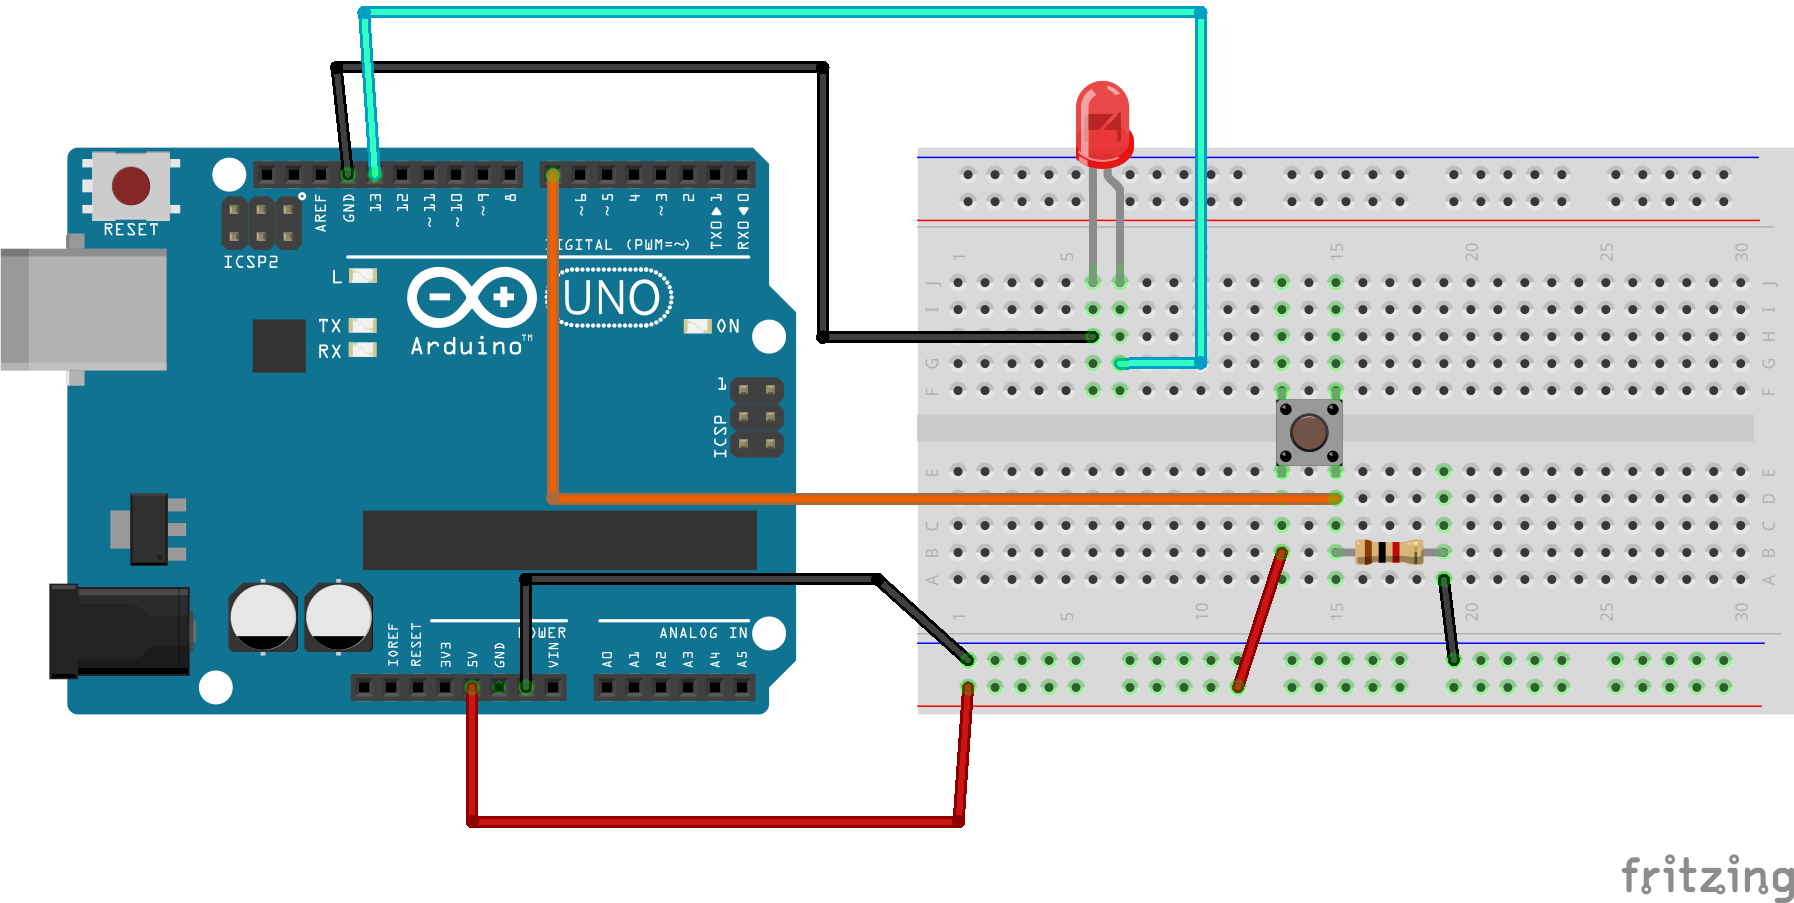
\includegraphics[scale=0.62]{immagini/schema_arduino.png}
	\caption{Esempio di schema creato con Fritzing. Rappresenta uno dei primi test effettuati con scheda Arduino.}
	\end{center}
\end{figure}

\medskip

%Il progetto verrà spiegato in questa sezione, senza però scendere in dettagli, evitando quindi riproducibilità.
Lo sviluppo del progetto è partito da uno studio preliminare sul sistema già esistente composto da una centralina di controllo ed un lettore di schede NFC.
Scendendo nei dettagli, la fase di studio è iniziata dalla centralina, composta da una scheda Arduino. Per poterne apprendere il funzionamento, il tutor aziendale mi ha fornito una scheda di test sulla quale eseguire del codice di esempio con dei semplici circuiti elettronici. L'apprendimento si è rivelato piuttosto rapido anche grazie alla vasta disponibilità di materiale online e ad una consolidata community.

Una volta appreso il funzionamento generale di Arduino, ho iniziato lo studio sul codice che governa il comportamento della centralina di controllo, caratterizzato principalmente da 3 fasi:

\begin{itemize}
\item \textbf{Configurazione iniziale}: il sistema esegue una configurazione iniziale in modo da integrarsi perfettamente nella rete alla quale è collegato;
\item \textbf{Listener}: una porzione di codice che rimane in continuo ascolto per catturare gli eventi derivanti dai moduli collegati;
\item \textbf{Crittografia e HTTP request}: una funzione che si occupa della cifratura dei codici letti e del loro invio tramite richieste HTTP ad un server.
\end{itemize}

Terminata questa prima fase di studio, è susseguita quella di analisi.

\section{Analisi dei requisiti}
\subsection{Identificazione}
Per poter identificare correttamente tutti i requisiti, a seguito di vari colloqui con il tutor aziendale e il cliente, ho definito i vari casi d'uso, disegnandone in seguito i rispettivi diagrammi UML. Ogni riunione è stata riportata su di un verbale e da quest'ultimo ho in seguito ricavato i vari requisiti. Ho anche analizzato approfonditamente i casi d'uso in modo da poter identificare ulteriori requisiti. Una volta individuati tutti i requisiti sono stati riportati in un documento soggetto a versionamento.

\subsection{Strumenti a supporto}
\subsubsection{Casi d'uso}
I casi d'uso e i relativi diagrammi UML sono stati un ottimo strumento di supporto durante la fase di analisi: mi hanno permesso di individuare alcuni requisiti non emersi durante le riunioni con tutor e stakeholders.

\begin{figure}[H]
	\begin{center}
	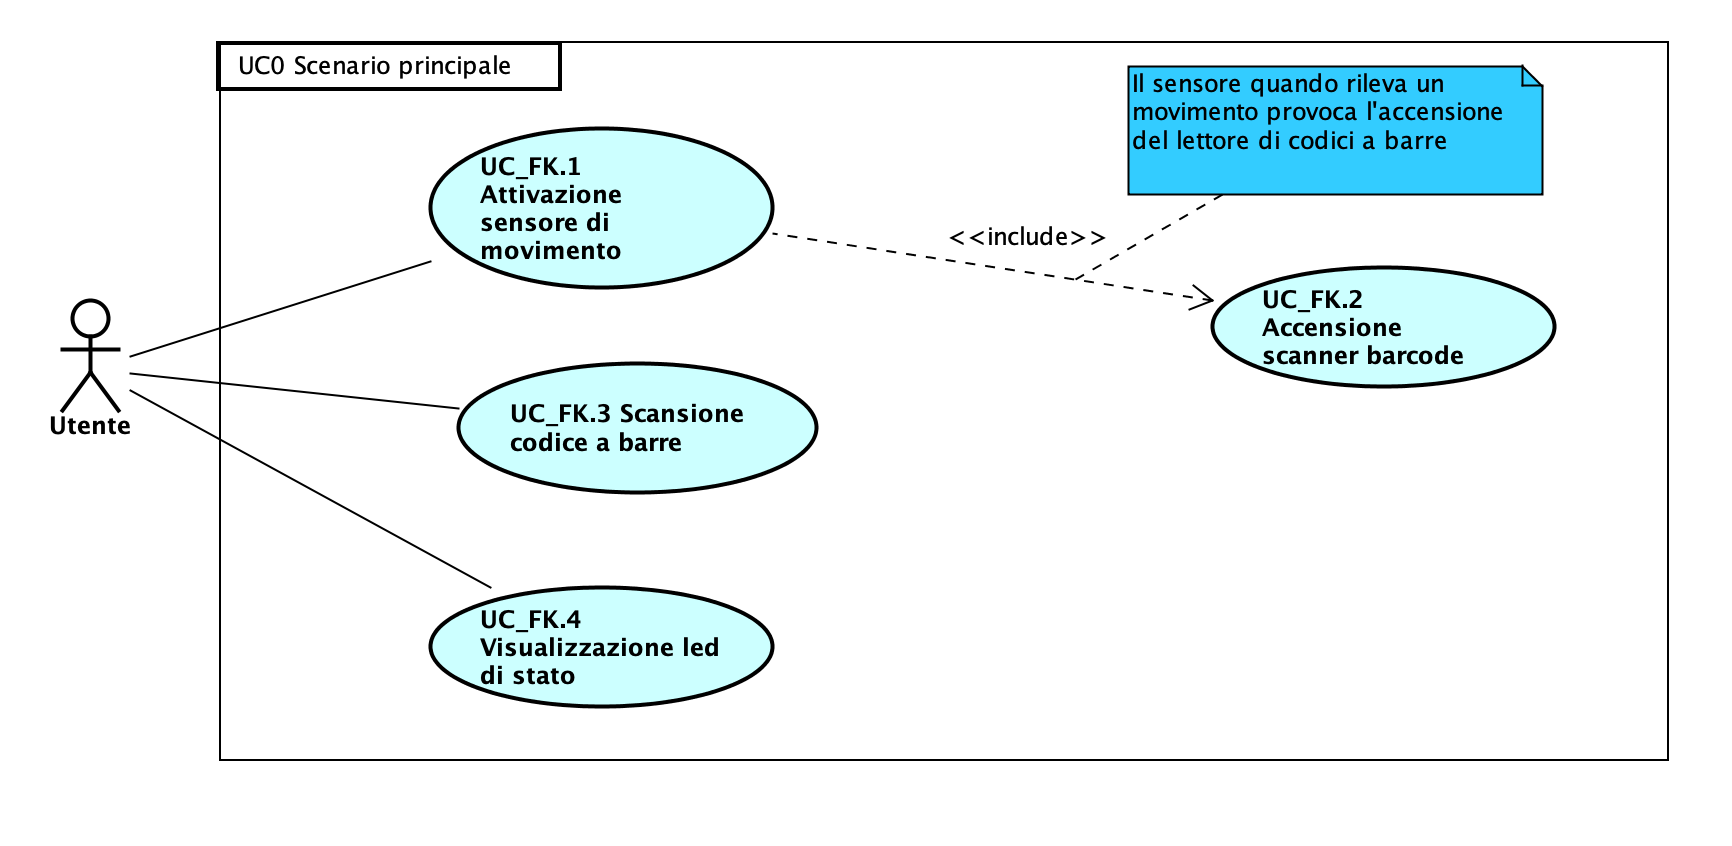
\includegraphics[scale=0.4]{immagini/usecase/scenario_principale.png}
	\caption{Estratto dello schema UML rappresentante i casi d'uso dello scenario principale. Schema riferito all'uso di FabKey e non alla piattaforma online.}
	\end{center}
\end{figure}

Essendo il progetto composto da due sistemi, FabKey e piattaforma online, i casi d'uso sono stati categorizzati da una notazione univoca, che facilita l'identificazione del caso d'uso nel contesto:

\begin{center}
\textbf{UC\textunderscore [Contesto].[IDUnivoco]}
\end{center}

\begin{itemize}
\item \textbf{Contesto}:
\begin{itemize}
\item \textbf{FK}: FabKey;
\item \textbf{PO}: Piattaforma online di gestione.
\end{itemize}

\item \textbf{IDUnivoco}: Un codice numerico progressivo che identifica in maniera univoca il caso d'uso a cui si riferisce. Questo codice può essere gerarchico in modo da identificare casi d'uso innestati.
\end{itemize}

\begin{figure}[H]
	\begin{center}
	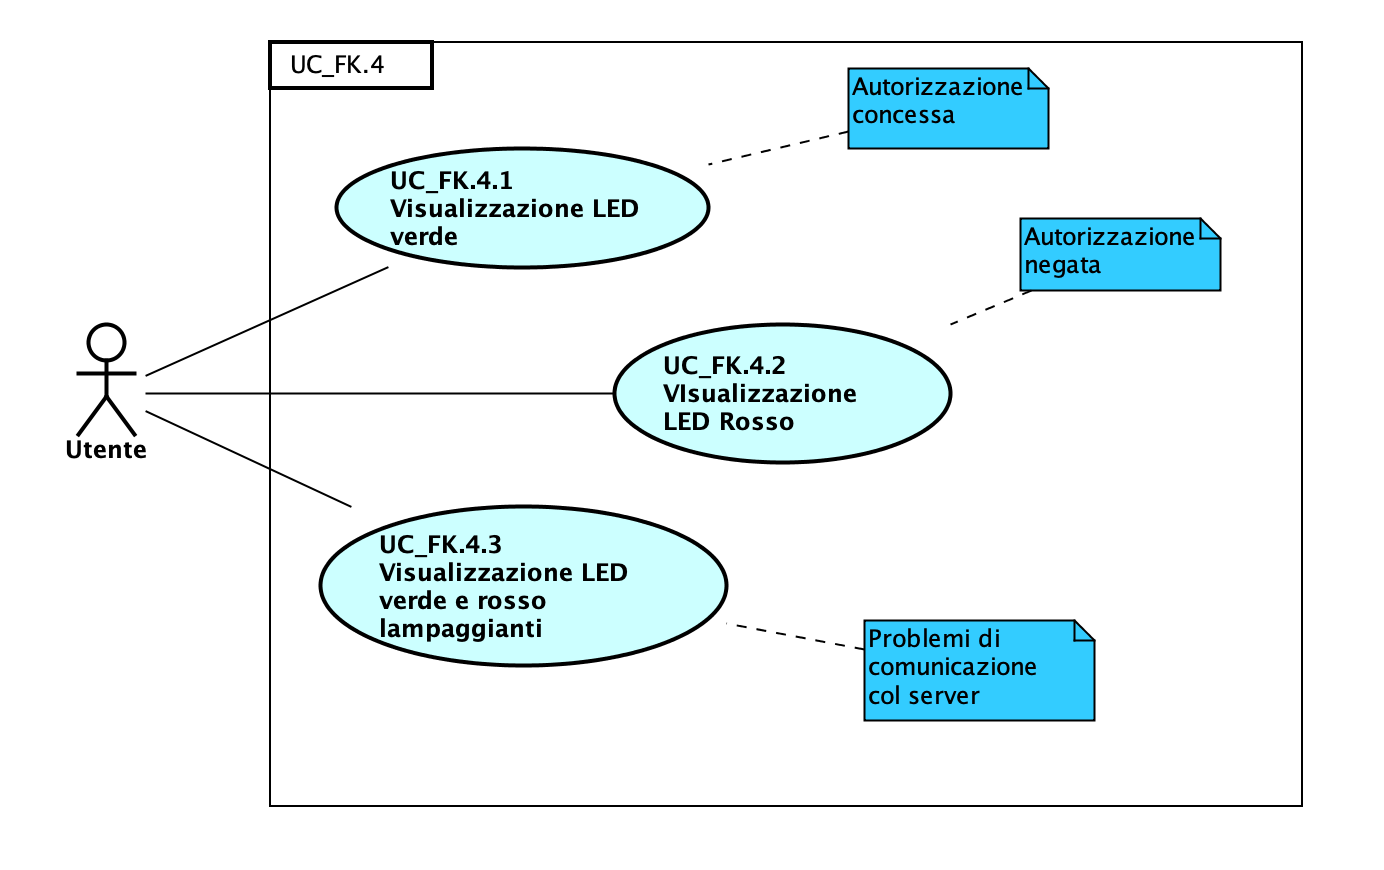
\includegraphics[scale=0.4]{immagini/usecase/UC_FK_4.png}
	\caption{Dettaglio del caso d'uso UC\textunderscore FK.4. Si può notare l'uso della notazione sopra descritta.}
	\end{center}
\end{figure}

Ogni caso d'uso ha una specifica provenienza, ovvero alcune determinate fonti che lo hanno generato.
Queste sono:
\begin{itemize}
\item \textbf{Verbali}: ottenuti trascrivendo quanto emerso durante i colloqui con i portatori di interesse;
\item \textbf{Le specifiche del sistema}: descrivono quali sono le caratteristiche che il sistema deve avere;
\item \textbf{Conoscenza del dominio}: la conoscenza del contesto d'utilizzo e la consultazione di materiale ad esso inerente.
\end{itemize}

Ho utilizzato queste fonti anche per l'identificazione dei requisiti.

\subsection{Formalizzazione dei requisiti}
Dopo aver individuato tutti i requisiti necessari allo sviluppo del progetto, ho creato una codifica che li potesse identificare in maniera univoca e allo stesso tempo catalogare per tipo e priorità.
La codifica utilizzata è la seguente:

\begin{center}
\textbf{R[Componente]\textunderscore [Tipologia]\textunderscore [Priorità][Numero Identificativo]}
\end{center}

\textbf{Componente}
\begin{itemize}
\item \textbf{FK}: requisito inerente allo sviluppo della parte elettronica di FabKey;
\item \textbf{PO}: requisito relativo allo sviluppo del portale online per la gestione degli accessi.
\end{itemize}

\textbf{Tipologia}
\begin{itemize}
\item \textbf{F}: un requisito di tipo funzionale, cioè che aggiunge funzionalità al sistema;
\item \textbf{Q}: requisito di qualità, ovvero che, se soddisfatto, aumenta la qualità generale del prodotto;
\item \textbf{P}: requisito prestazionale, mirato a migliorare il prodotto in termini di prestazioni.
\end{itemize}

\textbf{Priorità}
\begin{itemize}
\item \textbf{Ob}: requisiti obbligatori, il cui sviluppo è condizione necessaria per ottenere il risultato finale;
\item \textbf{De}: requisiti desiderabili, ovvero soddisfarli significa apportare importanti miglioramenti al prodotto anche se non strettamente vincolanti al suo funzionamento;
\item \textbf{Op}: requisiti opzionali, che apportano valore aggiunto al sistema, ma il cui sviluppo è trascurabile.
\end{itemize}

\textbf{Numero Identificativo}

\medskip

Un codice numerico progressivo che identifica in maniera univoca il requisito a cui si riferisce. Questo codice può essere gerarchico.

\bigskip

Riporto di seguito alcuni dei requisiti individuati:

\medskip

\textbf{Hardware FabKey}
\renewcommand{\arraystretch}{2.0}
\begin{longtable}{|l|p{2.5cm}|p{8cm}|}
\hline
\textbf{Codice} & \textbf{Tipo} & \textbf{Descrizione} \\ 
\hline
\textbf{RFK\_F\_Ob1} & Funzionale \linebreak Obbligatorio & Il sistema deve permettere la lettura di un codice a barre \\ 
\hline
\textbf{RFK\_F\_Ob2} & Funzionale \linebreak Obbligatorio & Il sistema deve attivare il lettore quando rileva un utente nelle vicinanze \\
\hline
\textbf{RFK\_Q\_Ob1} & Qualità \linebreak Obbligatorio & Il modulo di lettura deve essere contenuto in un involucro stampato in 3D \\
\hline
\textbf{RFK\_Q\_Op1} & Qualità \linebreak Opzionale & L'involucro esterno deve essere modulare ed espandibile per versioni successive \\
\hline
\end{longtable}


\medskip

\textbf{Portale online}
\renewcommand{\arraystretch}{2.0}
\begin{longtable}{|l|p{2.5cm}|p{8cm}|}
\hline
\textbf{Codice} & \textbf{Tipo} & \textbf{Descrizione} \\ 
\hline
\textbf{RPO\_F\_Ob1} & Funzionale \linebreak Obbligatorio & L'applicazione deve permettere di visualizzare l'elenco degli utenti autorizzati \\ 
\hline
\textbf{RPO\_F\_Ob2} & Funzionale \linebreak Obbligatorio & L'applicazione deve permettere di gestire le autorizzazioni \\
\hline
\textbf{RPO\_F\_Ob2.1} & Funzionale \linebreak Obbligatorio & L'applicazione deve permettere di eliminare un'autorizzazione \\
\hline
\textbf{RPO\_F\_De1} & Funzionale \linebreak Desiderabile & L'applicazione deve presentare un'interfaccia grafica completamente scalabile \\
\hline
\end{longtable}


Dopo aver individuato e codificato tutti i requisiti, ho composto una tabella in cui ho riportato il tracciamento tra i requisiti e i casi d'uso, in modo da identificare in quale caso d'uso viene soddisfatto un determinato requisito.

\section{Progettazione}
Ho gestito la progettazione del prodotto in modo separato rispetto alle due componenti principali che ne fanno parte: l'hardware di FabKey (composto da centralina e lettore) e l'applicazione online per la gestione delle autorizzazioni. Per comodità chiamerò queste due componenti \textbf{HWFabKey} e \textbf{Gestionale accessi} rispettivamente.

\medskip

La fase di progettazione è stata molto importante, in quanto la sua corretta realizzazione mi avrebbe permesso una fase di codifica rapida minimizzando i rischi di errore.

\bigskip

\textbf{Progettazione di HWFabKey}

\begin{figure}[H]
	\begin{center}
	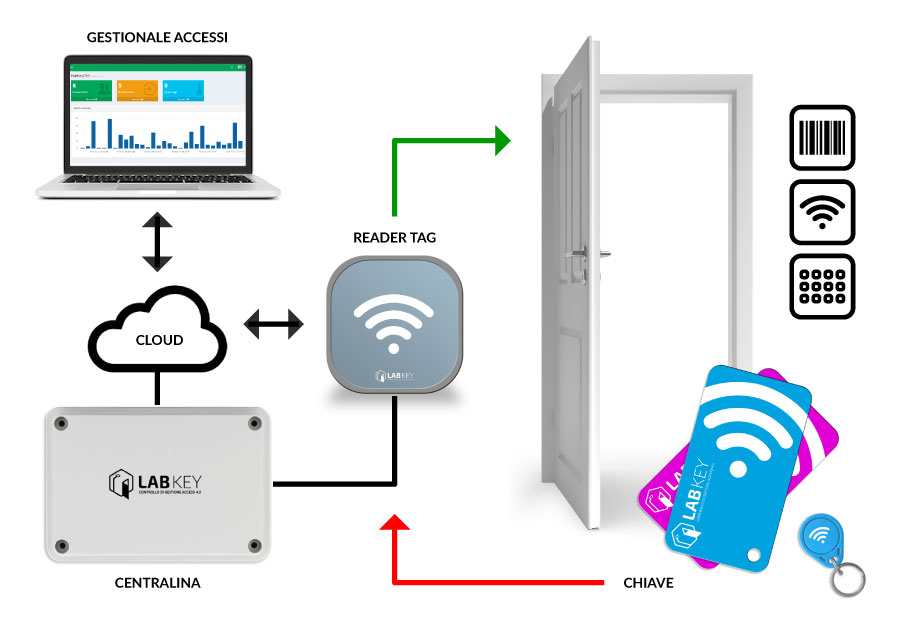
\includegraphics[scale=0.4]{immagini/schema_labkey.jpg}
	\caption{Schema di funzionamento di FabKey.}
	\small{\textbf{Fonte:} \url{https://www.labkey.it}}
	\end{center}
\end{figure}

%Progettazione online app
% Si potrebbe inserire un grafico che rappresenti il database MySql
%ragioni della scelta del db relazionale

\section{Codifica}

\section{Verifica e validazione}

\section{Visione generale del progetto}